\documentclass{article}

\usepackage{natbib}
\usepackage{authblk}
\usepackage[utf8]{inputenc}
\usepackage{hyperref}
\usepackage{graphicx}
\usepackage{multirow}
\usepackage{tabularx}
\usepackage{booktabs}
\usepackage{longtable}
\usepackage{appendix}
\usepackage{xcolor}
\usepackage{booktabs} 

\usepackage{times}
\usepackage{latexsym}
\usepackage{floatpag}

\usepackage[parfill]{parskip}
\usepackage[utf8]{inputenc} % allow utf-8 input
\usepackage[T1]{fontenc}    % use 8-bit T1 fonts
\usepackage{hyperref}       % hyperlinks
\usepackage{url}            % simple URL typesetting
\usepackage{booktabs}       % professional-quality tables
\usepackage{amsfonts}       % blackboard math symbols
\usepackage{nicefrac}       % compact symbols for 1/2, etc.
\usepackage{microtype}      % microtypography
\usepackage{graphicx}
\usepackage{natbib}
\usepackage{tabularx}
\usepackage{xtab}

\usepackage{float}   % For the [H] specifier to force placement


\usepackage{geometry}  %this makes the columns wider 
\usepackage{siunitx}
\usepackage{booktabs, makecell}
\usepackage[referable]{threeparttablex}

\title{%The KL3M Dataset:  A Copyright Clean 80TB+ Dataset for Pretraining and Supervised Fine Tuning of Language Models

The KL3M Dataset:  A Copyright Clean 80TB+ Dataset for Pretraining and Supervised Fine Tuning of Large Language Models


}
\author{\normalsize{Michael J Bommarito II,\textsuperscript{1,2} Jillian Bommarito}\textsuperscript{1} \& Daniel Martin Katz\textsuperscript{1,2,3,4}\\
  \textit{\small \textsuperscript{1} Institute for the Advancement of Legal and Ethical AI (ALEA Institute)\\
  \textit{\small \textsuperscript{2} CodeX -- The Stanford Center for Legal Informatics}\\
  \textit{\small \textsuperscript{3} The Law Lab, Illinois Tech - Chicago Kent College of Law}\\          
    \textit{\small \textsuperscript{4} Center for Legal Technology \& Data Science, Bucerius Law School}\\  
  }
}
  
\date{\normalsize{March 13, 2025}}

\begin{document}

\maketitle

\begin{abstract}
{Practically all large language models have been pre-trained on data that is subject to global uncertainty related to copyright infringement, breach of contract, and privacy. In light of this reality, we present the 80TB+ sized Kelvin Legal Large Language Model (KL3M) dataset, the largest collections of pretraining and supervised fine-tuning data which is unencumbered by copyright risk.  In total, KL3M contains over 125 million documents and more than 1.7 trillion tokens.  This paper outlines our approach to creating a dataset free from copyright uncertainty including details on our data sources, and collection and preprocessing methods.  While our data sources are limited to US and certain EU source materials, we open source not only the dataset itself but also the tokenizer, API's and other associated software in order to support further allied development in other jurisdictions.  We believe that this represents a significant step towards developing A.I. systems that are legally and ethically sound, both now and in the face of future regulatory changes.}
\end{abstract}
\section{Introduction}
Over the past decade, there has been significant progress on general-purpose language modeling driven by the application of neural based methods \cite{rumelhart1986learning}\cite{hopfield1982neural} to corpora of increasing larger scales.\cite{brown2020language}\cite{dubey2024llama}\cite{guo2025deepseek}  Leading large language models (LLMs) have displayed significant progress on a range of challenging real-world tasks.\cite{goh2025gpt}\cite{dell2023navigating}\cite{katz2024gpt}\cite{brin2023comparing}

While fewer and fewer question the technical progress of these models' capabilities, the training and use of large language models, however, is not without controversy.   Indeed, there are an emerging range of questions associated with the development of generative A.I. technology.  These objections vary and cover a range of topics including the `openness' of the model creation process and the `toxicity' of the subsequent outputs.\cite{liesenfeld2024rethinking}\cite{longpre2024pretrainer}\cite{bommasani2024foundation}  While these are certainly important issues, far less attention, by contrast, has been paid to use training data collected at scale without respect to the moral and legal rights of its creators.  

Virtually all existing LLMs rely upon the large-scale collection and use of materials that are subject to copyright. Despite various clever efforts to ameliorate such issues at both training \cite{minsilo2024} and inference time \cite{golatkar2024cpr}\cite{ippolito2023preventing}\cite{flemings2024differentially} many leading models can still engage in relatively high levels of potentially infringing behavior.\cite{chen2024copybench}     

There is still the open question of whether notions ``fair use" or ``fair dealing" might serve as a legal defense to this otherwise problematic behavior.\cite{henderson2023foundation}\cite{sag2024fairness}  However, it is worth noting that while ``[M]ore than forty countries with over one-third of the world’s population have fair use or fair dealing provisions in their copyright laws,"\cite{band2013fair} the interpretation of such principles can vary significantly across jurisdictions.\footnote{It is worth noting that although some model providers are offering ``fair use'' as a defense to their data collection practices, many such organizations are also inherently acknowledging the property rights of creators by entering into licensing deals.} 

In light of this reality, we set out on an alternative path - one that is rooted in a rigorous data collection and curation processes designed to respect traditional legal and ethical frameworks.  In this paper, we present the Kelvin Legal Large Language Model (KL3M) dataset, tokenizer, software, and APIs. These assets, open-sourced and maintained by the ALEA Institute,\footnote{\textit{See} Institute for the Advancement of Legal and Ethical AI (ALEA Institute) \url{https://aleainstitute.ai/} } represent one of the largest collections of pretraining and supervised fine-tuning data unencumbered by copyright risk.  We outline a framework for determining permissibility of content usage that can be employed by anyone who wants to gather or audit training data for model training or fine-tuning. In addition, we enhance the data provenance visibility of the KL3M dataset by providing Dublin Core metadata for all data in the dataset.\cite{park2009dublin}

%Thus, in the following sections, we will detail our data sources, collection process, preprocessing methods, and the characteristics of the resulting dataset. We will also discuss the implications of our work for future A.I. development in the context of the broader legal and ethical landscape.



%Our approach aims to circumvent the need for reliance on fair use arguments by ensuring all data in the KL3M dataset is either in the public domain or explicitly licensed for unrestricted use.

%In light of this reality, we set out on an alternative research agenda - one that is rooted in legal and ethical practices that are free of doubt. Our primary contribution to a space already saturated with datasets is the research into and development of a path that is free of reliance on the "fair use" argument that is often relied upon for model training.


%With over 30 copyright lawsuits against AI companies currently in progress in the US alone, the need for legal precedent on the matter of copyright infringement and model training is clear. The outcome of these cases will likely establish whether the argument for "fair use" in model training is a viable one. 

%However, regardless of what one believes about the legal and ethical questions underlying this uncertainty, there is no denying the existence of the many lawsuits and investigations ongoing in major jurisdictions.

\section{Copyright and Generative A.I.}
\subsection{Brief Overview of Copyright}
Copyright is sometimes described as a `bargain’ where creators receive, exclusive rights to their works for a specific period of time, in exchange for the public eventually gaining free access to those works after the copyright term expires.\cite{patterson1991nature} Although all materials will eventually reach the public domain, creators may, during their period of exclusive ownership, choose to make their works available to others via licensing at a scope of their choosing.  There is a wide continuum of popular copyright licenses including MIT, Apache, GNU GPL, AGPL as well as various flavors of Creative Commons licenses.\cite{metzger2015free}  Such licenses provide a wide degree of latitude for creators to control the scope of how their respective works are used.  

In the internet era, many individuals and organizations have chosen to make their otherwise copyrighted works available online for the scope delimited use of others. Through various platforms such as \textit{Github} (computer code), \textit{Getty Images} (image licensing), \textit{YouTube} (video repositories) or directly through personal websites, the internet has arguably facilitate the most extensive period of information sharing in all of human history.  At the same time, there have also been disputes surrounding the extent to which digitized information could be made available to users. Indeed, controversy has been `part and parcel' of the internet era including major clashes over projects such as \textit{Google Books}\cite{samuelson2009google} and file sharing sites such as \textit{Napster}.\cite{rayburn2001after}  

\subsection{Copyright and A.I. Data Collection}
Although disagreement over proper the scope of copyright is not new, the advent of LLMs has brought with it heightened concerns about the acquisition and use of otherwise copyrighted source materials.\cite{samuelson2023generative}  Virtually all model providers and large scale datasets collected in furtherance of building LLMs have ignored both the website terms of service in the scraping of websites as well as licensing restrictions attached to the respective content collected.\cite{longpre2024large}  As a result, the internet has seen a rise in restrictions upon sharing including a range of efforts to prevent data from being used in the training of A.I. systems.\cite{longpre2024consent}  
Individual creators and content based organizations threatened by A.I. systems that arguably undermine creators future economic prospects have begun to place additional restrictions on their works in an effort to limit reuse, redistribution, and commercial use of their copyrighted materials in the building of A.I systems.\cite{longpre2024consent}

Since the advent of the large-scale public internet, there have been a variety of public and commercial efforts to track its development and growth.\cite{mcmurdo1995internet}\cite{alnoamany2014and}  Much of those efforts centered around ``search'' and helping route individuals to relevant webpages. However, indexing the internet is not the precisely akin to full collection of content.  For example, in the early years of the current millennia, linguists were slow to include large-scale web content given anxiety over copyright in the underlying source materials.\cite{ide2002american}  While some of such materials did eventually make their way into important corpora,\cite{ide2008american} the specter of legal restrictions caused some to limit their use of materials obtained from the internet. 

Other groups, however, were far less motivated by such concerns and began to look at the internet as a premier source of data.  Beyond mere tracking and indexing, internet data has been subjected to various large scale collection efforts including graph data, images, metadata and the underlying text.\cite{buck2014n}\cite{leskovec2016snap}\cite{deng2009imagenet}  \textit{Common Crawl}\cite{smith2013dirt} one of longest standing efforts to collect web-scale data has served as a foundational dataset in many early LLMs. \textit{Common Crawl} and subsequent efforts to build large-scale A.I. training datasets such as the \textit{Colossal Cleaned Common Crawl} (C4)\cite{raffel2020exploring}, \textit{The Pile}\cite{gao2020pile} and \textit{Dolma}\cite{soldaini-etal-2024-dolma} are replete with copyrighted data. 

%Common Crawlhas been cited in thousands of academic articles \footnote{https://github.com/commoncrawl/cc-citations/} 

As noted earlier, the collection and distribution of such materials relies upon ``fair use'' as a justification. ``Fair use'' is fact-specific inquiry meaning that whether a particular use of copyrighted material is considered ``fair use'' depends upon specific details that must be evaluated on a case-by-case basis.  For example, when an academic institution or other non-profit type research organization collects data for research purposes that activity would likely be ``fair use.''  Yet, if that same dataset were deployed for subsequent commercial use by an entity whose direct or indirect aim is to undercut the commercial viability of the original creator (\textit{e.g.} coder, artist, author or musician) that activity might not be characterized as ``fair use.''  Even if ``fair use'' were not deemed to cover a particular usage, it is possible that royalty system including perhaps compulsory licensing might be a vehicle for rewarding creators\footnote{A market based licensing and royalty system including perhaps a compulsory licensing would be more ethical than allowing individuals and organizations to seize the creative works of others without \textit{any} compensation. Such ideas are explored in a recent report released by the U.S. Copyright Office.\cite{Jaffe2025}} while still allowing for innovation in A.I. model building to continue.\footnote{In a letter sent to the White House Office of Science and Technology (OSTP), OpenAI argued that ``[A]pplying the fair use doctrine to AI is not only a matter of American competitiveness — it’s a matter of national security ... If the PRC’s developers have unfettered access to data and American companies are left without fair use access, the race for AI is effectively over.''\cite{OpenAI}  While clarity regarding the legal treatment of this question would be helpful, it is far from clear that the requirement of royalty payments to creators would materially impair the rate of innovation.}

Certain scholars working with datasets such as \textit{Common Crawl}, \textit{C4} and \textit{The Pile} have recognized the looming copyright questions surrounding these efforts.\cite{schafer2016commoncow}\cite{habernal2016c4corpus}  For example, authors of the recently released  \textit{Dolma} dataset stated ``that the legal landscape of A.I. is changing rapidly, especially as it pertains to use of copyrighted materials for training models.''\cite{soldaini-etal-2024-dolma}  However, they still chose to distribute their dataset because the ``sources were publicly available and already being usedin large-scale language model pretraining (both open and closed).'' 

This perspective is emblematic of much of the broader literature on ethics in A.I. where there has been much greater focus on questions of model ‘openness’ and `A.I. alignment' than respect for the scope of the moral and legal rights of creators.  Although issues of transparency and model toxicity are important, they are far from the only consideration worthy of attention.  

Most recently, the \textit{Common Corpus} dataset\cite{arnett2024toxicity}  was released on the \textit{Hugging Face} platform.  The dataset was promising as the authors claimed that the compilation ``contains only data that either is uncopyrighted or permissively licensed.''  Unfortunately, the rhetoric surrounding the dataset does not match its reality.  Although the authors recognize the ethical and potential legal issues associated with scraping data without the consent of the data creator, the authors provide very little description of their copyright audit process.  It turns out that even a cursory inspection of the dataset reveals a significant volume of copyright materials contained therein. 


%As noted earlier, the extant literature has in part begun to acknowledge and confront some of the potential ethical and legal challenges associated with the construction of modern LLMs. Much of the focus, however, has been directed at questions of model ‘openness.’   While ‘openness’ is certainly an attractive property of a development pipeline, it is insufficient without a clear analysis of the ethical and legal requirements.  

%by contrast, does not even pretend to care about the rights of content creators.  Instead, it is includes components such as Books3, Pile-CC, Github and Wikipedia.   FOOTNOTE  [[ The use of Wikipedia (whose pages feature a wide range of licenses selected at the behest of users) is almost certainly problematic at scale.  The Wikimedia foundation lacks the legal authority to change the license terms for  ]]


%As noted earlier, the extant literature has in part begun to acknowledge and confront some of the potential ethical and legal challenges associated with the construction of modern LLMs. Much of the focus, however, has been directed at questions of model ‘openness.’   While ‘openness’ is certainly an attractive property of a development pipeline, it is insufficient without a clear analysis of the ethical and legal requirements.  

%The authors of Common Corpus dataset recognize that it is unethical (and arguably illegal) to scrape (data) without the consent of the data creator.   While the authors claim that the dataset ‘contains only data that is uncopyrighted or permissively licensed,’ the authors provide no description of the process by which such copyright analysis was conducted.  And in fact, even a minimum inspection reveals a significant amount of copyright materials contained with the dataset.   

%The Pile, by contrast, does not even pretend to care about the rights of content creators.  Instead, it is includes components such as Books3, Pile-CC, Github and Wikipedia.   FOOTNOTE  [[ The use of Wikipedia (whose pages feature a wide range of licenses selected at the behest of users) is almost certainly problematic at scale.  The Wikimedia foundation lacks the legal authority to change the license terms for  ]]

   





\section{Copyright Clean Collection Process}
We believe that the continued development and use of AI systems should be predicated on such systems being both legally and ethically compliant, both in the current environment and in the wake of future regulatory and legislative changes.  In this section, we introduce the Kelvin Legal Large Language Model (KL3M) dataset, the largest dataset developed to date that respects the moral and legal rights of copyright holders. Our approach aims to circumvent the need for reliance on ``fair use" arguments by ensuring all data in the KL3M dataset is either in the public domain or explicitly licensed for unrestricted use.


\subsection{Copyright Filtration Process}
To build KL3M, we developed a multi-part filtration process designed to determine whether a given data source may be used without significant restriction. The test is based on a series of conditional assessments: if the data passes a test, we include it in the KL3M dataset; if the data does not pass the test, we move on to the next test. Data that does not pass any of our tests is not included in the KL3M dataset.  We describe the process below but also highlight the steps in Figure \ref{fig:CopyrightFlowchart} below.

\begin{figure}[ht!]
\centering
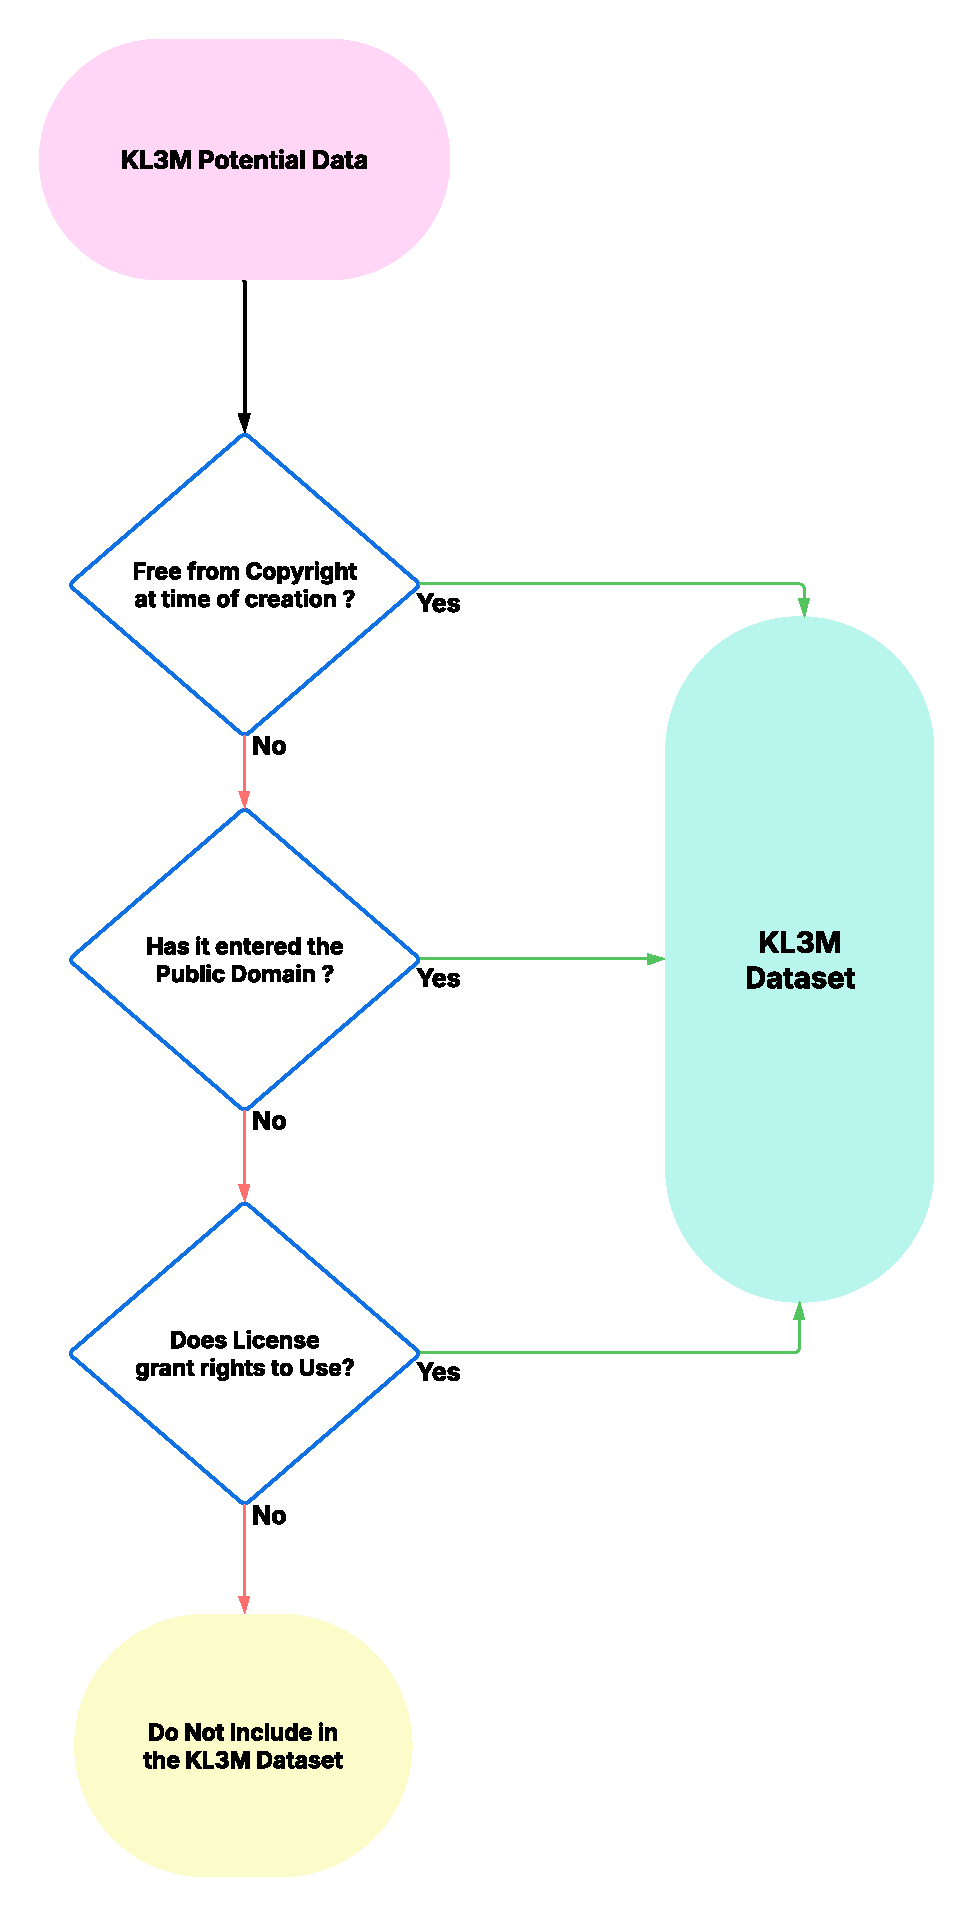
\includegraphics[width=70mm]{CopyrightFlowchart.pdf}
\caption{Overview of the Copyright Filtration Process}
\label{fig:CopyrightFlowchart}
\end{figure}

\subsubsection{Test 1 - Free from Copyright Protection}
Our first test is to determine whether the content is free from copyright \textbf{at the time of its creation}. A substantial percentage of content contained within the KL3M dataset meets this test and was thus eligible for inclusion.

Works of the United States government, for example, are not eligible for copyright protection under 17 U.S.C. § 105 (``Copyright protection under this title is not available for any work of the United States Government").  Specifically, work created by a federal government employee or officer is in the public domain, provided that the work was created in that person’s official capacity. 

A separate but related concept is the ``government edict doctrine."  This doctrine, developed through the common law, denies copyright protection to official ``government edicts."\footnote{The doctrine is long standing and dates back to \textit{Wheaton v. Peters}, 33 U.S. (Pet. 8) 591 (1834) and has most recently been addressed in \textit{Georgia v. Public.Resource.Org, Inc.}, 590 U.S. 255 (2020).}  The doctrine exists to effectuate the principle that citizens must have unrestrained access to the laws that govern them.  The ``government edict doctrine" allows for the publication of various legislative and judicial pronouncements including judicial opinions.  As noted by the U.S. Copyright Office, the doctrine extends to ``all legislative enactments, judicial decisions, administrative rulings, public ordinances, or similar types of official legal materials.''\footnote{U.S. Copyright Office, Compendium of U.S. Copyright Office Practices, §313.6(C)(2) (3d ed. 2017)}

Most but not all countries follow this doctrine. For example, we had hoped to include certain UK legal sources within the KL3M dataset but limitations embedded in the Open Justice License (OJL)  surrounding the ``computational analysis of the information'' prevented us from including such UK data at this time.\footnote{\textit{See} Open Justice License (OJL) \url{https://caselaw.nationalarchives.gov.uk/open-justice-licence}} 

\subsubsection{Test 2 - Public Domain Materials}
In our second test, we determine whether content has \textbf{entered into the public domain} or its equivalent, such as a Creative Commons - No Rights Reserved (CC0) license where no rights are reserved. There are several ways that content, once subject to copyright, could thereafter enter the public domain.  Most notably, although the amount of time has changed over the years, copyright is always a temporary grant of exclusive rights for a defined period of time.  Therefore, once that designed time has lapsed, the work automatically enters the public domain.  For example, while we would prefer to include the most recent Twelfth Edition\cite{black2024} published in 2024, we instead include in the KL3M data the Second Edition of Black's Law Dictionary originally published in 1910.\footnote{Black's Law Dictionary contains definitions of specialized legal terms. The substantive meaning of many such terms has not changed for many years.} 

Other information can enter the public domain as part of a particular legal process.  For example, we include granted patents in KL3M as patents are typically not subject to copyright restrictions.  As noted by the USPTO, ``[P]atents are published as part of the terms of granting the patent to the inventor.''  Absent a limited set of circumstances, ``the text and drawings of a patent are typically not subject to copyright restrictions.''\footnote{\textit{See} USPTO Terms of Service \url{https://www.uspto.gov/terms-use-uspto-websites}}  
%Following the terms We include also include public comments on regulatory submissions as part of notice and comment rule making within the KL3M dataset. 

One additionally important vehicle for adding information to the public domain is the US Federal Depository Library Program (FDLP). The Federal Depository Library Program (44 U.S.C. § 19), administered by the U.S. Government Publishing Office, was established to ensure that the American public has access to Government information. 44 U.S.C. § 1911 states that ``[D]epository libraries shall make Government publications available for the free use of the general public.''  Although many of the documents required extensive pre-processing in order to be usable, the FDLP is a very large source of useful information for KL3M.  

\subsubsection{Test 3 - Minimally Encumbered Content with Clear Rights to Copy, Modify, and Redistribute}
If the use of content is not otherwise permissible following the two prior tests, the final test is to determine whether the \textbf{license attached to the content grants a user the right to copy, modify, and redistribute the content without significant restriction}.  As highlighted in Figure \ref{fig:CopyrightFlowchart}, if content fails this final test, we did not include it in the KL3M dataset.

While CC0 or No Rights Reserved is, of course, the most unencumbered form of license, there are a range of other content licenses that might theoretically be considered for inclusion.   Overall, we evaluated content with the following license types using the reasoning below:

\begin{itemize}
\item CC0: included given content is shared with No Rights Reserved 
\item CC BY: included as the attribution is not overly burdensome (particularly in the case of an institution as author)
\item CC BY-SA: excluded due to the uncertainty around meeting share-alike obligations in the context of a Large Language Model\footnote{While we plan to meet the Share-alike requirements in the full Open Source release of KL3M, we recognize that others might consider this to be major encumbrance upon utilization.}
\item CC BY-NC: excluded due to non-commercial limitation
\item CC BY-NC-SA: excluded due to non-commercial limitation and uncertainty around meeting share-alike obligations
\item CC BY-ND: excluded due to limitation on derivative work
\item CC BY-NC-ND: excluded due to non-commercial and derivative work limitations
\end{itemize}

In general, in the context of content created by an institution, we believe an attribution requirement is only a very modest restriction upon downstream use.  For example, content released by the European Commission under 2011/833/EU is only minimally encumbered as it merely imposes an ``obligation for the reuser to acknowledge the source of the [Commission's] documents.''\footnote{\textit{See} On the reuse of Commission documents \url{https://eur-lex.europa.eu/eli/dec/2011/833/oj/eng}}  Similarly, in most cases, compliance with the attribution requirement set forth in the Creative Commons License (CC BY) is similarly straightforward.  

However, there are arguably some nuances and complexity in the context of non-institutional authors. Indeed, some of the most fruitful data that we might consider for inclusion could not meet our goal of building a dataset that was relatively unencumbered.  For example, despite its inclusion in other training datasets such as \textit{Colossal Cleaned Common Crawl} (C4) \cite{raffel2020exploring}, \textit{The Pile} \cite{gao2020pile}, \textit{Dolma} \cite{soldaini-etal-2024-dolma} and \textit{Common Corpus} \cite{arnett2024toxicity}, \textit{Wikipedia} and many other knowledge commons are arguably encumbered by the ``copyleft'' licenses that the community has chosen. 

From a historical perspective, \textit{Wikipedia} content was originally licensed under the GNU Free Documentation License  (GFDL).\cite{roessing2010authorship}  Today, it is arguably licensed under CC BY SA which carries with it not only a share alike (SA) requirement but also an attribution requirement (BY).  We contacted the \textit{Wikimedia Foundation} to ascertain their perspective regarding the scope of attribution that they believe would be required to use the content on \textit{Wikipedia}.  Specifically, given the millions of total contributors who at some point have authored content on \textit{Wikipedia}, we wanted to determine whether they believe that a general attribution statement or a specific attribution statement was required.   

In the context of building or fine-tuning large language models, a general attribution statement highlighting the respective input sources to a given dataset or model is relatively easy to provide.  However, specific attribution to the specific work or works that gave rise to a \textit{specific model output} is a difficult if not impossible technical challenge. It was the Wikimedia Foundation's position that ``providing a general notice to customers would not be an adequate solution to compliance.''  While Wikimedia's interpretation of the CC BY SA requirement is not the final word on this important legal question, we did feel comfortable including this content given it would significantly encumber downstream usage.\footnote{It is not clear how \textit{any} model creator could comply with a \textit{specific attribution} requirement given current technical limitations. At best, one could construct a system to assign \textit{statistical attribution} by assigning attribution through some sort of 
potential \textit{n-gram} based matching or other higher-order statistical style inference.  However, from an attribution perspective, this would undoubtedly produce false positives as well as false negatives.}  

In addition to the Wikimedia Foundation's interpretation of the (BY) requirement, \textit{Wikipedia} has a share alike (SA) requirement which like other ``copyleft'' licenses carries with it the requirement that downstream users make any new works they create with the original content available on the same terms as the original content.\cite{carver2005share}\cite{lessig2004creative} Specifically, the human-readable summary of the \textit{Wikipedia Creative Commons Attribution-ShareAlike 4.0 International License} states ``if you alter, transform, or build upon this work, you may distribute the resulting work only under the same, similar or a compatible license.''\footnote{\textit{See} Wikipedia Creative Commons Attribution-ShareAlike 4.0 International License \url{https://en.wikipedia.org/wiki/Wikipedia:Text_of_the_Creative_Commons_Attribution-ShareAlike_4.0_International_License}} Given these restrictions, it is unclear how \textit{any} model creator could use \textit{Wikipedia} data without making their model fully available under similar CC BY SA / GFDL terms.\footnote{Relying solely on the ``fair use,'' virtually \textit{all} model providers have used \textit{Wikipedia} data in constructing their models. To our knowledge, however, none of them have followed the attribution requirement (BY) as interpreted by the \textit{Wikimedia Foundation} and most do not come close to complying with \textit{Share Alike} (SA) requirement.}  

%\footnote{Similarly, the Wikipedia Creative Commons Attribution-ShareAlike 3.0 International License states ``If you remix, transform, or build upon the material, you must distribute your contributions under the same license as the original.} 

%It should be noted that book platforms such \textit{OpenStax} have similar issues where many individual authors have selected licenses that significantly impair subsequent use.   

%While institutional attribution requirements for content such as EU sources under 2011/833/EU, providing a general notice to customers would not be an adequate solution to compliance. 

%Unlike the institutional attribution requirements for content such as EU sources under 2011/833/EU, copyleft licenses such as GNU FDL and CC BY SA.

%While the United Kingdom's Open Government License (OGL) appears to also have only limited restrictions, access to case law falls under the Open Justice License (OJL).  As noted above the presence of the ``computational analysis'' clause counseled us against including such information.  

%\subsection{Technical Description}
% Add details about the technical process of retrieving the texts here when available

\subsection{Fairly Trained Certification}
In 2024, the KL3M dataset was audited by the independent non-profit \textit{Fairly Trained}.\footnote{\textit{See} Fairly Trained \url{https://www.fairlytrained.org/} }  \textit{Fairly Trained} is a non-profit certification and auditing organization supported by many creators which is devoted to the certification of models that uphold the highest standards of respect for copyright.  

In certifying a model or dataset as \textit{Fairly Trained}, we were required to provide the provenance of each source contained within the dataset including a detailed review of our KL3M Copyright filtration process.  In addition, we needed to demonstrate any models or libraries we leveraged in the data collection, curation, processing steps were also not built upon the unauthorized use of third party content. After an extensive audit process, the KL3M dataset was the first large language model dataset ever to be certified as \textit{Fairly Trained}.   




%\textcolor{red}
%{DISCUSS KL3M vs other datasets on ALEA Site and the idea that the audit caused us to remove things -- podcasts, certain UK Data, etc. }
%\textcolor{black}

\subsection{Personal Information Considerations}
Personal information instances within the KL3M dataset generally arise from their inclusion in documents that are a matter of the public record or that are works of the government. As a result, the personal information that could theoretically be obtained through a review of the KL3M dataset is already publicly available.

We follow the approach of \textit{CourtListener} and the Board of Directors of \textit{The Free Law Project}.\footnote{\textit{See} CourtListener \url{https://www.courtlistener.com/} and the Free Law Project \url{https://free.law/}} in managing the tension between privacy and the public interest. Documents are only removed from the database under explicit court order.

\subsection{Current Jurisdictional Coverage of KL3M}
We chose to focus on content regulated by US and EU law due to our familiarity with these jurisdictions and the legal intricacies of intellectual property rights. We recognize that this limited coverage does not address much of the world's population and languages, but we hope that the process and tests that we have outlined in this paper as well as the associated infrastructure we have open sourced will enable others to create similar datasets for additional jurisdictions.



%\subsection{Regulatory Compliance Considerations}
%Add text about how this dataset will better enable developers to meet regulatory obligations, particularly with respect to transparency
\section{Overview of KL3M Collection Process}
In developing the Kelvin Legal Large Langugage Model (KL3M), we sought to collect and curate a large body of information which was free from the specter of copyright infringement. As opposed to broad data collected from the internet writ large, we sought to identify sources of high quality information, free from copyright concerns that were reasonably available online.  Governmental data, thus currently represents the vast majority of data within the Kelvin Legal Large Language Model (KL3M) dataset. As an output of the growth of the modern regulatory state,\cite{katz2020complex}\cite{coupette2021measuring} various components of government produce very large bodies of relatively high-quality information content.  In addition, various legal and regulatory processes require individuals and organizations to draft and submit various forms of information to government officials, often with guidance and oversight by lawyers, accountants and other professionals.  
%This led us to primarily focus on information produced by or otherwise made available by government(s) as among other things such data is much higher quality than typical internet data.  

While the substantive quality of many forms of governmental data is quite high, the organization and accessibility of such information is not always nearly as strong.  Although governmental and other related data has slowly made it way into the digital world, the mere digitization of governmental information or work product has not always allowed the public to obtain the crucial information they need.  Poorly designed websites, a lack user-friendly navigation and outdated and inconsistent digital platforms are just some of the challenges faced by individuals engaging with public sector information systems.  We faced these very challenges in collecting and curating the KL3M dataset. Although much of this data is theoretically accessible, it is often stored in various inconsistent formats which make cross-functional access very difficult even in discrete amounts (let alone at scale). 

In this section, we begin by discussing trends in modeling building while providing some exemplars of the wide-ranging content contained within the KL3M dataset.  Next, we detail our efforts to collect, pre-process and organize this vast and diverse corpora.  Finally, we provide a high level overview of the distribution of sources contained within the current version of the Kelvin Legal Large Language Model (KL3M) dataset. 
  
\subsection{Breadth and Quality of Tokens Might Be What You Need}
One challenge in building modern language models is to have both scale and a diversity of pre-training information content to cover the broad conceptual space of potential user queries.  Users might want to ask a model to explain a scientific question, determine how best to cook a particular recipe, look to draft some long-form prose or perhaps even ask questions about how to sublease their apartment.  The prevailing approach to cover the broad conceptual space of potential user queries is simply to scale models to increasing large scales.\cite{kaplan2020scaling}  ``Chinchilla'' and other related scaling laws have encouraged model builders to pre-train on the maximal amount of available pretraining data.\cite{hoffmann2022training}\cite{pearce2024reconciling}.  As such, most developments in LLMs have been focused on the use of various collections of internet and so called ``publicly available'' data to build larger and larger language models. 

Undoubtably, the sheer power of scale has delivered some fairly remarkable results. Engineering, however, is not only about performance, it is also about cost.\cite{Krishna2025}  Thus, an alternative strain of work has focused upon how to cost effectively train models using distillation and other related techniques.\cite{guo2025deepseek}\cite{zhang2024tinyllama}\cite{javaheripi2023phi} The scaling laws upon which the field was once fixated have arguably given way to a more nuanced perspective where token diversity, token quality and test time inference scaling are also an important part of the overall calculus.\cite{snell2024scaling}\cite{yu2024makes}  

\subsection{The Incredible Expanse of Government Work Product}
Legal and regulatory processes implicate a wide variety of pursuits and fields of human endeavour.  Thus, taken as a whole, the work product of governments and governmental processes covers a significant amount of intellectual territory.  While certainly not covering every topic that a user might find interesting, information from governments covers a surprising amount of the broader conceptual space.  Laws, regulations, scientific reports, food safety bulletins, environmental impact assessments, public health guidelines, statistical reports, press releases, disaster preparedness plans, government contracts and certain private contracts, judicial opinions, public commentary, military directives, food and drug recalls, transportation safety reports, economic forecasts, patent filings, congressional testimony, securities filings, census data reports are just some examples of the outputs associated with the governmental work product and governmental processes.  

KL3M features a wide variety of question and answer pairs, professional dialogues, formal definitions of key terminology and parallel assessment documents in multiple languages.  It is quite difficult to fully characterize the incredible expanse of topics and materials contained therein.  Appendix I highlights the KL3M Data Gallery, an online exploration tool which allows users to review millions of sample documents drawn from the broader KL3M dataset.  However, consider Figure \ref{fig:KL3MImages} which offers just a few selected examples that are exemplars of the broader set of data contained in KL3M.  Across the four examples, we observe a wide range of topics from turducken food handling, micronutrient testing in vitamins and carotenoids, mineral resources of the Owyhee River Canyon in Idaho and an analysis of the change in input impedance for electrically short dipole antennas.  Agencies represented such as the United States Department of Agriculture, NIST, Department of Commerce and the Department of Interior are just a small subset of the total agencies producing government work product on a daily basis.

\begin{figure}[H]
\centering
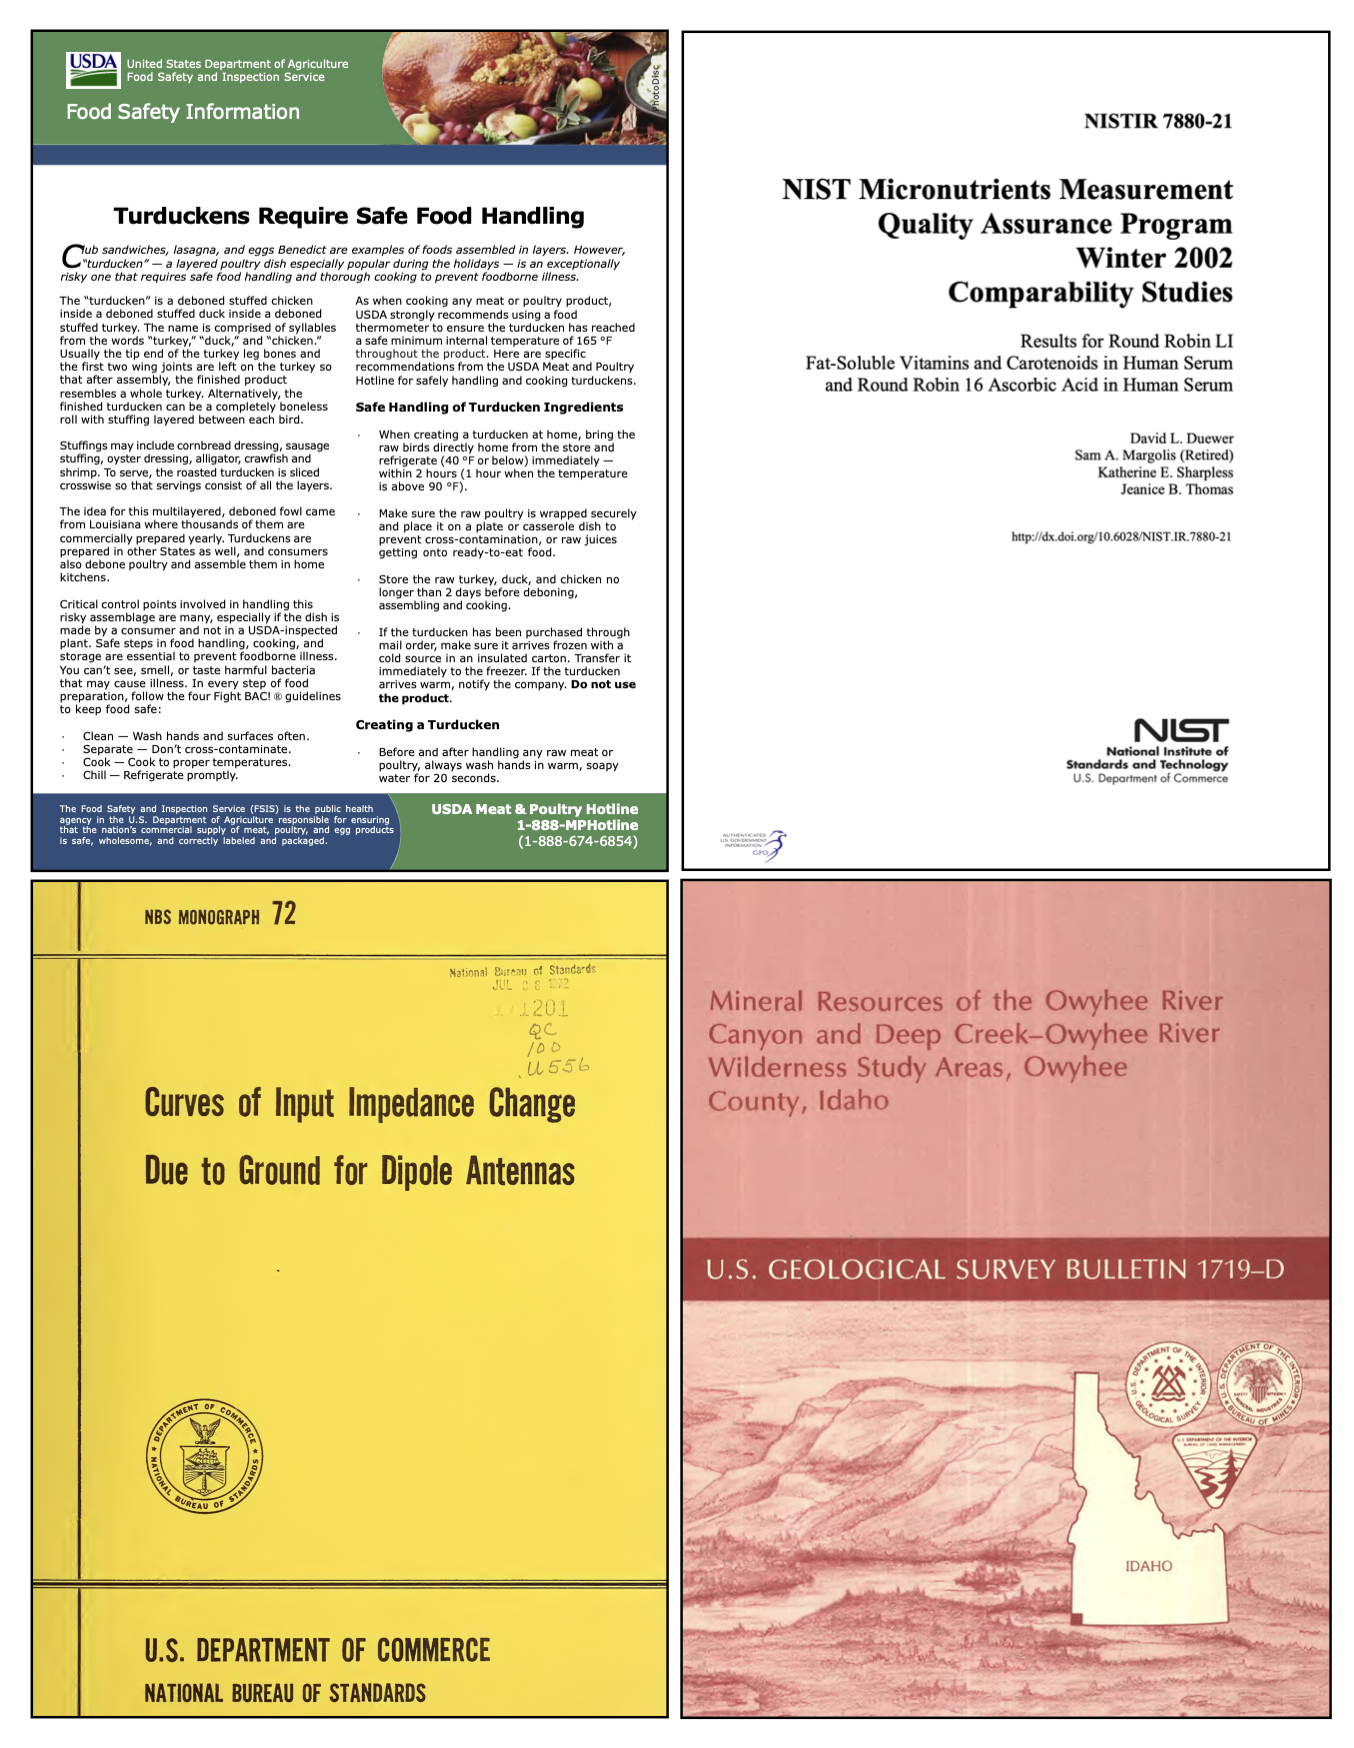
\includegraphics[width=95mm]{KL3MImages.png}
\caption{\centering{Samples of Content from the KL3M Dataset}}
\label{fig:KL3MImages}
\end{figure}

\subsection{The Collection \& Pre-Processing Data Pipeline for KL3M}
Working with the vast array of document types such as those displayed in Figure \ref{fig:KL3MImages} is a challenging proposition.  To do so effectively at scale, we developed a pre-processing pipeline designed to engage with the real-life challenges associated with the unstructured, inconsistent and complex forms of documents across the various information systems with which we engaged.  Thus, in addition to the KL3M dataset, we are also releasing all of the tooling and libraries leveraged across the KL3M Pre-Processing pipeline as it is our hope that others might adapt this work in order to build parallel corpora in other jurisdictions.   

\begin{figure}[h!]
\centering
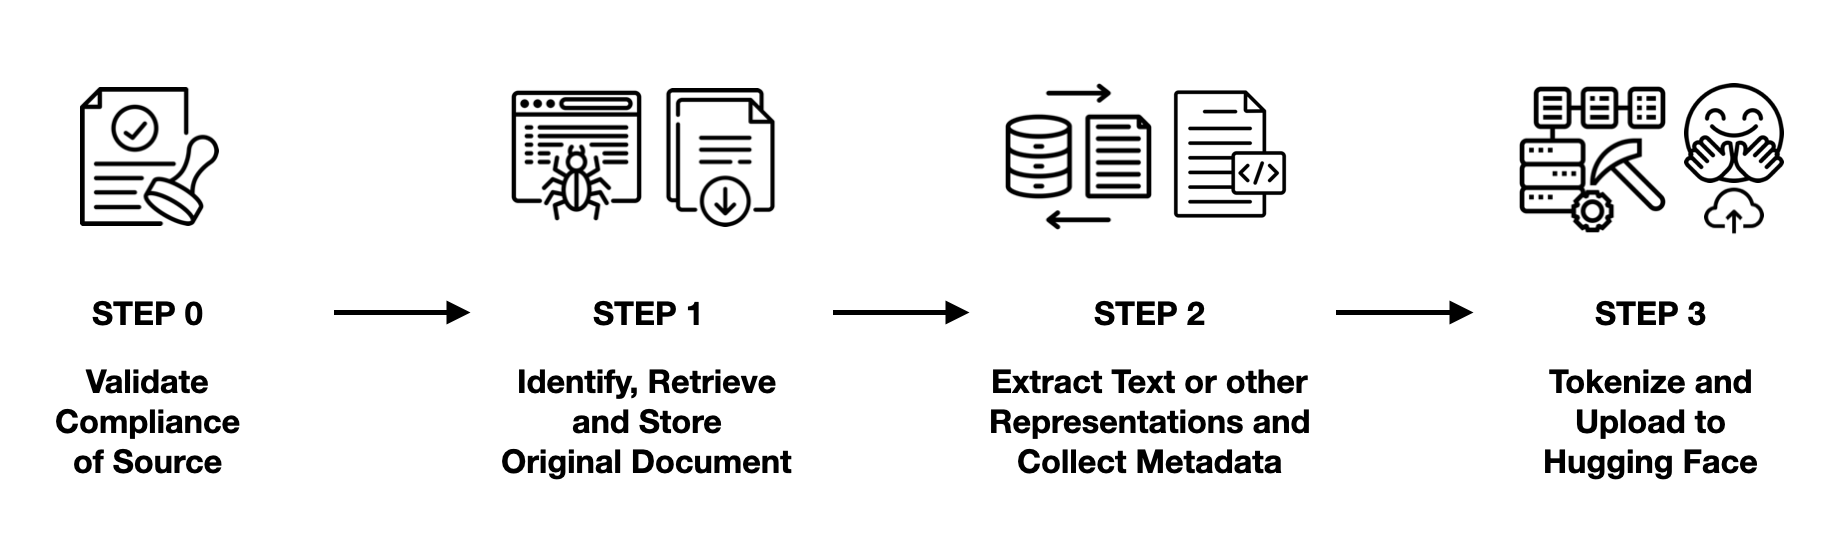
\includegraphics[width=150mm]{PreProcessing.png}
\caption{\centering{{Overview of the Pre-Processing Pipeline} - (icons via Flaticon)}}
\label{fig:preprocessing}
\end{figure}


Figure \ref{fig:preprocessing} provides a high-level overview of our pre-processing pipeline.  Building from our copyright filtration process described in Figure \ref{fig:CopyrightFlowchart}, we begin by identifying a potential source of useful content.  Next, we must determine whether that candidate source complies with our requirements. Thus, \textit{Step 0} is high level recitation of the process described in Figure \ref{fig:CopyrightFlowchart}.  Having then identified and validated compliance of the source material, we next proceed to \textit{Step 1} of Figure \ref{fig:preprocessing} where we retrieve and retain the original source material for provenance purposes.\footnote{This ability to demonstrate original source provenance was critical in obtaining the \textit{Fairly Trained} Certification described in Section 3.2.}  

In \textit{Step 2}, we develop an alternative representation of the documents which varies depending upon the nature of the original source.  Our ideal path is to build an alternative representation of all source materials in Markdown \cite{mailund2019beginner} while also retaining the original source material in parallel.  However, this is not always possible given the nature of the original source.  Finally, in \textit{Step 2} were also collect and store \textit{Dublin Core Metadata} for all source material.  

In \textit{Step 3}, we tokenize all objects using a custom tokenizer developed specifically for this task.  The KL3M tokenizer has several specific elements that makes it unique \color{red}\textbf{[MIKE ADD HERE 2-3 sentences]} \color{black}  Finally, we upload the tokenized document to their respective folder on \textit{Hugging Face}.\footnote{The KL3M Data can be access here \url{https://huggingface.co/collections/alea-institute/kl3m-data-679f9db9b6fd93f91c3c633e}}


%\section{Pre-Processing}
% Add details about the pre-processing steps applied to the data
\section{Dataset Characteristics}

\subsection{KL3M Components and Summary Statistics}
While currently limited mostly to governmental sources, the KL3M dataset features a relatively large and diverse set of content such as the content highlighted in Figure \ref{fig:KL3MImages}.  In Table \ref{table:summarystats}, we present summary statistics for the overall dataset.  In total, the KL3M dataset features more than 125 million documents, 1.7 trillion tokens and more than 80 terabyte of total information content.  

\begin{table}[!htbp]
    \small
    \centering
    \begin{tabularx}{0.6\linewidth}{X @{\hskip 3pt} l @{\hskip 3pt}}
        \toprule
        \textbf{KL3M Features} & \\
        \midrule
        Total Documents in KL3M & 126 Million Documents \\
        Total Tokens in KL3M  & 1.7 Trillion Tokens \\
        Total File Size & 80 Terabytes \\
        \midrule
        \bottomrule
    \end{tabularx}
    \caption{Summary Statistics for KL3M Dataset}
    \label{table:summarystats}
\end{table}

Given the range of sources as the vast interconnectedness of ideas, concepts, there is almost certainly duplicate content contained herein. A document may quote elements of other documents or otherwise incorporate concepts from other documents.  Thus, the overall token count is somewhat larger than if one were to consider something such as the total number unique n-gram combinations.  However, we did not deduplicate the underlying content as we envision a wide range of potential uses for this overall source material.  Downstream users can thus decide how to mix, match, segment or further pre-process the content in order to support their specific objective or use case.  

\begin{table}[!htbp]
   \footnotesize
  \centering 
    \begin{tabular*}{\linewidth}{Xlrrr|r}
    \toprule
    \textbf{KL3M Component}  & {\sc{File Size}} & {\sc Document Count} & {\sc Token Count} & {\sc Avg Token Per Doc}\\
    \midrule
    Securities \& Exchange Commission Filings & 00.0GiB & 0.0 & 0.0 & 0.0 \\
Congressional Documents & 00.0GiB & 0.0  & 0.0 & 0.0 \\
Congressional Bills & 00.0GiB & 0.0  & 0.0 & 0.0 \\
Code of Federal Regulations &  00.0GiB & 0.0 & 0.0 & 0.0 \\
Electronic Code of Federal Regulations &  00.0GiB & 0.0  & 0.0 & 0.0  \\
Federal Depository Library Program &  00.0GiB & 0.0 & 0.0 & 0.0  \\
Federal Register &  00.0GiB & 0.0  & 0.0 & 0.0 \\
Federal Judicial Center &  00.0GiB & 0.0 & 0.0 & 0.0  \\
CIA World Factbook &  00.0GiB & 0.0  & 0.0 & 0.0  \\
Congressional Research Service &  00.0GiB & 0.0 & 0.0 & 0.0 \\
United States Government Manual &  00.0GiB & 0.0 & 0.0 & 0.0 \\
Library of Congress - Country Profiles &  00.0GiB & 0.0 & 0.0 & 0.0 \\
Statutes at Large &  00.0GiB & 0.0  & 0.0 & 0.0 \\
Regulatory Submissions &  00.0GiB & 0.0 & 0.0 & 0.0 \\
United States Code &  00.0GiB & 0.0 & 0.0 & 0.0 \\
Court Documents - Opinions &  00.0GiB & 0.0 & 0.0 & 0.0 \\
Court Documents - Motions, Orders, etc. &  00.0GiB & 0.0 & 0.0 & 0.0\\
Court Documents - Dockets  &  00.0GiB & 0.0  & 0.0 & 0.0 \\
Black's Law Dictionary, 2nd Edition &  00.0GiB & 0.0 & 0.0 & 0.0 \\
U.S. Federal Government Websites &  00.0GiB & 0.0 & 0.0 & 0.0 \\
US Patent Grant Full Text Data &  00.0GiB & 0.0  & 0.0 & 0.0 \\
Official Journal of the European Union &  00.0GiB & 0.0 & 0.0 & 0.0 \\
    \midrule
    \textbf{Totals} & \textbf{0.0} & \textbf{0.0} & \textbf{0.0} & \textbf{0.0}   \\
    \bottomrule
    \end{tabular*}%
  \label{table:KL3M Components}%
      \caption{Summary Statistics of KL3M Components }
\end{table}

Table \ref{table:summarystats} displays the document counts, token counts and average tokens per document for each of the KL3M components.  While \textit{Securities \& Exchange Commission Filings} are the largest component of the dataset from a total documents and token perspective, there are some other large sources of input data.  Other large subset of data include [ FILL IN NEXT 3-4 items]  

Among some of the smaller KL3M components, there are interesting elements worthy of exploration including millions of conversational messages extracted from Congressional hearings, nearly 20 billion tokens worth of docket entiries 

Appendix II offers a more detailed description of each of the KL3M Components.  




\subsection{KL3M Additional Compositional Statistics}

\textbf{DISTRIBUTION OF DOCUMENT SIZE}

\begin{figure}[h!]
\centering
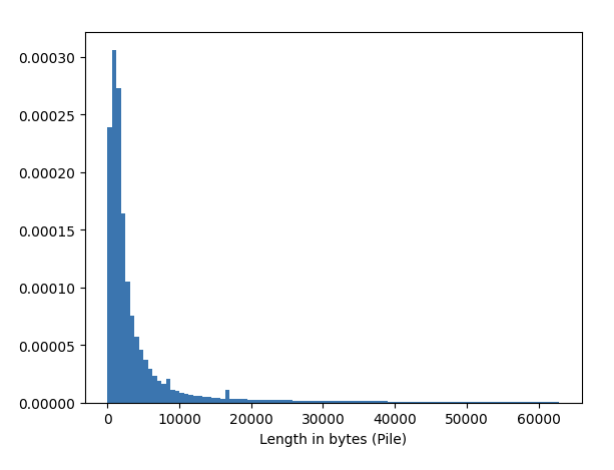
\includegraphics[width=90mm]{PileDist.png}
\caption{\centering{{Overview of the Pre-Processing Pipeline} - (icons via Flaticon)}}
\label{fig:Dist}
\end{figure}


\textbf{DISTRIBUTION OF PERPLEXITY SCORES}
\begin{figure}[h!]
\centering
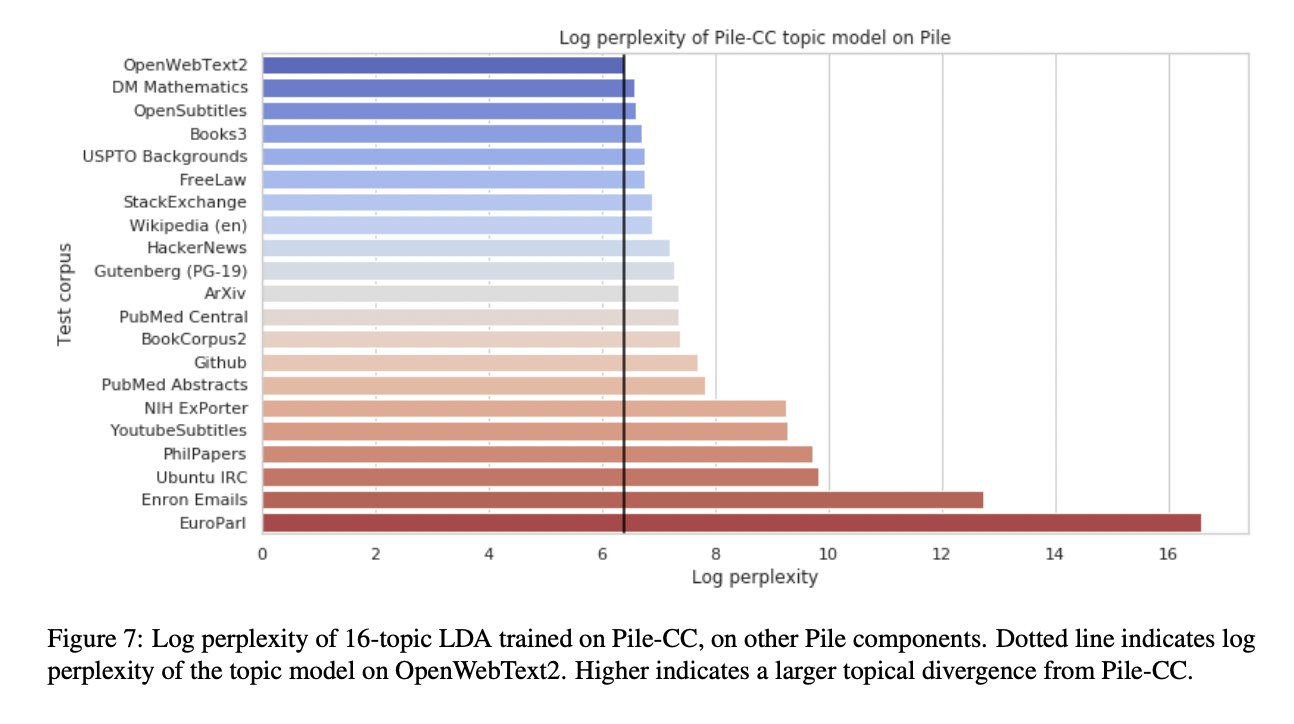
\includegraphics[width=110mm]{Perplexity.png}
\caption{\centering{{Overview of the Pre-Processing Pipeline} - (icons via Flaticon)}}
\label{fig:Perplexity}
\end{figure}


\textbf{TOXICITY ANALYSIS}
\begin{figure}[h!]
\centering
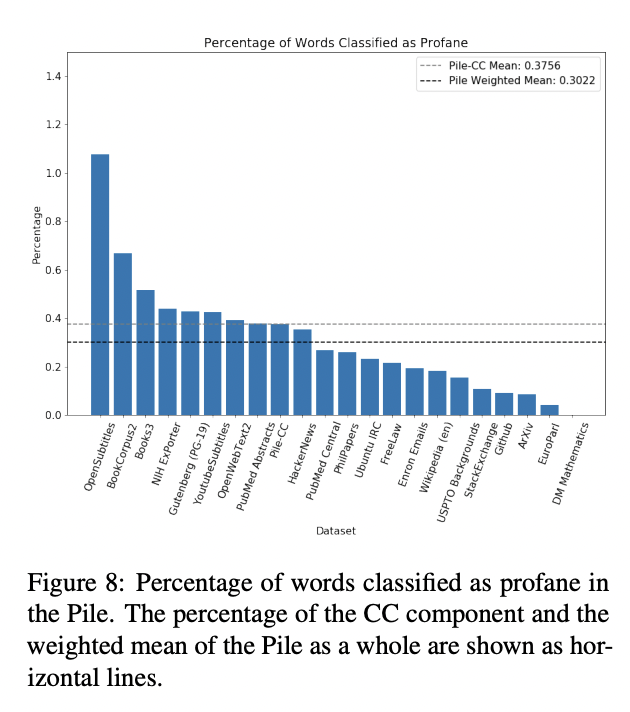
\includegraphics[width=90mm]{Toxicity.png}
\caption{\centering{{Overview of the Pre-Processing Pipeline} - (icons via Flaticon)}}
\label{fig:toxicity}
\end{figure}




Trying to copy some of the stuff reported in THE PILE paper 

\textbf{TOTAL TOKENS }

\vspace{10mm}

\textbf{TOTAL DOCS (with cavaet and discussion that doc is a tricky idea)}

\vspace{10mm}

\textbf{DISTRIBUTION OF TOKENS by Docs}

\vspace{10mm}

\textbf{SOME SORT OF TOKEN DIVERSITY MEASURE }

\vspace{10mm}





\textbf{Why US other countries -- data availability .. 
}





\section{A Living Dataset and Infrastructure for the Collecting and Distributing Copyright Clean Data}
In this paper, we introduced the Kelvin Legal Large Language Model (KL3M) dataset a large and diverse corpora of more than 125 million documents and more than 1.7 trillion tokens.  We describe our copyright filtration process designed to identify only source materials with clear provenance from a copyright perspective.  We then provided an overview of the pre-processing pipeline designed to 





The KL3M can be used in several ways.  First, it can serve as a baseline for model pretraining and could be combined with other appropriately license datasets.  Alternatively, it could be used to fine tune an existing model.  We realize that this dataset alone would likely be insufficent to allow for models to be built which cover the boundless set of possible use cases and user queries.  However, we believe this large body of tokens could be combined with selected forms of licensed content to develop LLMs which can deliver strong performance on certain tasks.  However, 
We believe that the development of datasets and models that are transparent, freely available without legal restrictions, and high quality will enable downstream use that is free of the infringement concerns often present.


The paper reflects the current version of the KL3M dataset as of the time of this publication.  Yet, rather than being a static snapshot, we hope that KL3M will persist as ``living dataset'' which we seek to update, maintain and extend as time moves forward.  In addition, we hope that KL3M will become a federated project where others leverage or retrofit some of our underlying infrastructure to expand the set of copyright clean data available from a global perspective.  

The KL3M dataset represents a significant step towards creating large language model training data that is free from copyright uncertainty. By carefully selecting and vetting our sources, we have created a resource that can be used with confidence by AI researchers and developers. We hope that our methodology will serve as a template for future efforts in this direction, ultimately leading to more legally and ethically robust AI systems.

As the field of AI continues to evolve rapidly, it is crucial that we address the legal and ethical challenges head-on. The KL3M dataset is our contribution to this effort, providing a foundation for the development of AI systems that can withstand future regulatory scrutiny and contribute positively to society.  While our focus has been on US and EU jurisdictions due to our familiarity with their legal systems, we recognize the need for similar efforts in other parts of the world. We encourage researchers and legal experts from other jurisdictions to adapt and expand upon our methodology to create globally representative datasets that are free from copyright concerns.

In conclusion, the KL3M dataset not only provides valuable training data for large language models but also sets a new standard for transparency and legal compliance in AI development. As we move forward, it is our hope that this work will inspire further innovation in the responsible and ethical advancement of AI technology.





\bibliographystyle{ieeetr}
\bibliography{article-min} 

\begin{appendices}

\pagebreak
\setcounter{secnumdepth}{0}
\appendix
\section{Appendix I}
\setcounter{secnumdepth}{0}
\large {\textbf{KL3M Data Gallery}}
\begin{figure}[h!]
\centering
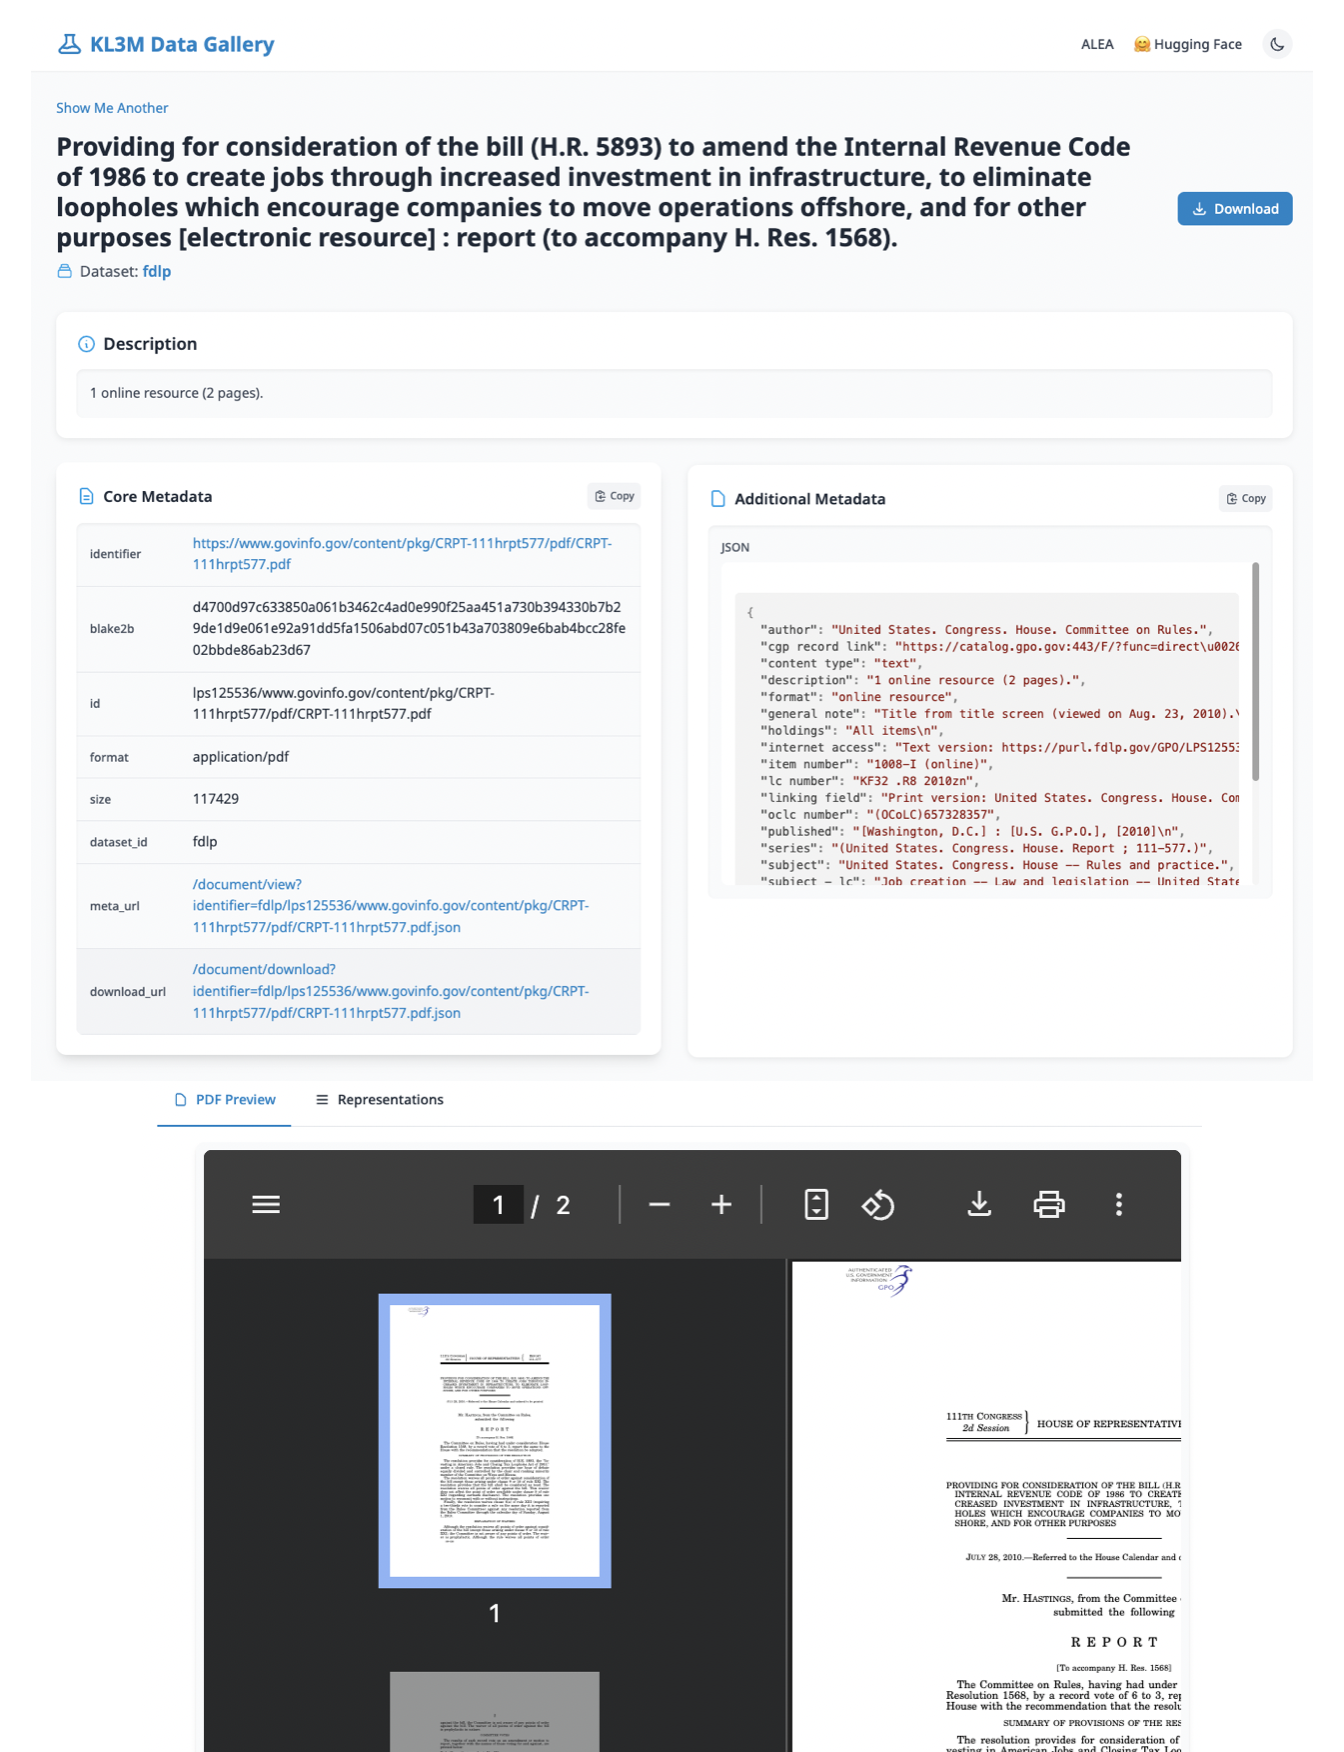
\includegraphics[width=120mm]{KL3MGallery.png}
\caption{\centering{KL3M Data Gallery - \url{https://gallery.kl3m.ai/}}}
\label{fig:method}
\end{figure}





\pagebreak
\section{\textbf{Appendix II}}
\setcounter{secnumdepth}{0}
\large {\textbf{KL3M Components Detailed Description}}
\begin{table}[h!]
\scriptsize
\begin{longtable}{ p{3cm} p{9cm} }
\textbf{KL3M Component}      
& \textbf{Description}  
\\\midrule
Securities \& Exchange Commission Filings & The U.S. Securities and Exchange Commission (SEC) is an independent agency of the federal government of the United States. As part of its role, the SEC requires public companies and other regulated entities to submit numerous filings and disclosures, which with limited exceptions (such as redacted information) are in the public domain. The KL3M dataset includes the following data subsets from the SEC: Public agreements, 10-K, 10-Q, 8-K, 6-K filings (foreign and domestic), Various S Filings, 6-K, 20-F, 40-F and associated exhibits and addenda.
\\
 \\\hline
 \\
Congressional Documents      
& The Congressional Documents Collection is a collection of various materials ordered to be printed by both the U.S. House and Senate. It is comprised of House Documents, Senate Documents, and Senate Treaty Documents. The House and Senate Documents contain various kinds of materials ordered to be printed by both chambers of Congress, including executive reports from agencies and departments. The Senate Treaty Documents contain treaty text as it has been submitted by the Senate for presidential ratification.
\\
 \\\hline
  \\
Congressional Bills &
This component includes legislative proposals within the United States Congress from the House of Representatives and Senate. This includes the entire life cycle of bills, from initial introduction to final published bills. 
\\   
 \\\hline
  \\
Code of Federal Regulations &
The Electronic Code of Federal Regulations (eCFR) is an editorial compilation of CFR material and amendments published in the daily Federal Register. The eCFR is continuously updated, but is not the official legal edition of the CFR. 
\\   
 \\\hline
  \\
Electronic Code of Federal Regulations &
The Electronic Code of Federal Regulations (eCFR) is an editorial compilation of CFR material and amendments published in the daily Federal Register. The eCFR is continuously updated, but is not the official legal edition of the CFR.   
\\   
 \\\hline
  \\
Federal Depository 
Library Program &
The Federal Depository Library Program (FDLP) provides a digitized record of the official documents published by the U.S. Government Publishing Office (GPO), GPO’s Superintendent of Documents, and other Federal agency publishers related to the FDLP.    
\\   
 \\\hline
  \\
Federal Register &
The Federal Register is the official daily publication for the following materials of the United States Federal Government: Presidential Documents, Executive Orders, proposed, interim, and final rules and regulations, and notices by Federal Agencies, as well as notices of hearings, decisions, investigations, and committee meetings. The National Archives and Records Administration is responsible for publishing the Federal Register.    
\\   
 \\\hline
  \\
Federal Judicial Center &
The Federal Judicial Center serves as the education and research agency for the U.S. federal courts. The KL3M dataset contains material published by the Federal Judicial Center, including research reports, monographs on substantive legal subjects, manuals, and reference guides.
\\
 \\\hline  
    \end{longtable}

\end{table}
\pagebreak

\begin{table}[h]
\scriptsize
\begin{longtable}{ p{3cm} p{9cm} }
\textbf{KL3M Component}      
& \textbf{Description}  
\\\midrule
\\
CIA World Factbook &
The World Factbook, developed by the U.S. Central Intelligence Agency (CIA), provides basic intelligence on the history, people, government, economy, energy, geography, environment, communications, transportation, military, terrorism, and transnational issues for 265 world entities.   
\\   
 \\\hline
  \\
Congressional Research Service    
& The Congressional Research Service (CRS) is a U.S. federal legislative branch agency that provides research services exclusively to congressional committees and Members of Congress. CRS reports, which are available to the public, cover a broad range of topics and are intended to reflect objective, nonpartisan research and analysis.
\\
 \\\hline
  \\
United States Government Manual &
The U.S. Government Manual is a regularly updated special edition of the Federal Register. Its contents include leadership tables and descriptions of agency activities and programs of the executive, judicial, and legislative branches of Federal U.S. Government, as well as those of quasi-official agencies and international organizations in which the United States is a participating member.
\\   
 \\\hline
  \\
Library of Congress - Country Profiles &
This collection of nearly 50 country profiles of foreign nations provides brief, summarized information on each country’s historical background, geography, society, economy, transportation and telecommunications, government and politics, and national security. This series of profiles is a subset of the Country Studies Program, formerly the Army Area Handbook Program. The collection was written between 2004 and 2008 and has not been updated since then.  
\\   
 \\\hline
  \\
Statutes at Large &
The United States Statutes at Large is the permanent collection of all laws and resolutions enacted during each session of Congress. The Statutes at Large is prepared and published by the Office of the Federal Register (OFR). The printed edition of the Statutes at Large is legal evidence of the laws, concurrent resolutions, proclamations by the President, and proposed and ratified amendments to the Constitution.  \\   
 \\\hline
  \\
Regulatory Submissions &
Any member of the public may submit comments on U.S. federal regulation through the website regulations.gov. The KL3M dataset contains the documents submitted as attachments to public comments. \\   
 \\\hline
  \\
United States Code &
The United States Code is a consolidation and codification by subject matter of the general and permanent federal laws of the United States. It is prepared by the Office of the Law Revision Counsel of the United States House of Representatives.
\\   
 \\\hline
  \\
Court Documents - Opinions &
U.S. federal and state court opinions are written explanations from judges that explain their decision and the facts and legal reasoning supporting it. The KL3M dataset contains court opinions obtained from two sources: PACER and CourtListener.  \\
 \\\hline
    \end{longtable}

\end{table}
\pagebreak


\begin{table}[!ht]
\scriptsize
\begin{longtable}{ p{3cm} p{9cm} }
\textbf{KL3M Component}      
& \textbf{Description}  
\\\midrule
\\
Court Documents Motions, Orders, etc. & Non-opinion court materials, such as motions, orders, and depositions were obtained through PACER. The non-opinions included in the KL3M dataset reflect content from federal courts only.   \\\\
 \\\hline
 \\
\textcolor{red}{\textbf{Court Documents - Dockets}}  
& 
\textcolor{black}{}\textbf{FILL THIS HERE}

\\
 \\\hline
  \\
Black's Law Dictionary, 2nd Edition &
The second edition of ``A Law Dictionary'' by Henry Campbell Black, commonly known as "Black's Law Dictionary" is a legal dictionary published in 1910 that contains definitions of the terms and phrases of both ancient and modern American and English jurisprudence \\\\
 \\\hline  \\
U.S. Federal Government Websites &
The KL3M dataset includes filtered content from websites of Federal agencies and departments of the United States. The content was filtered to limit inclusion to only that which is in the public domain.  \\
 \\\hline
 \\
US Patent Grant Full Text Data &
The United States Patent and Trademark Office (USPTO) publishes the full text, images/drawings, and complex work units (tables, mathematical expressions, chemical structures, and genetic sequence data) of each patent that is granted. The KL3M dataset only contains the full text of granted patents.
  \\
 \\\hline 
 \\
 Official Journal of the European Union &
The Official Journal of the European Union is the official publication for EU legal acts, other acts and official information from EU institutions, bodies, offices and agencies. \\
 \\\hline
    \end{longtable}

\end{table}

\end{appendices}

\end{document}



